% !TEX root =../main.tex

\chapter{Theoretischer Hintergrund und Konzepte}


\section{Definition vom Social Network}

Nach Charu C Social Network Data Analytics  (Seite 2 )„ in general, a social network is defined as a network of interactions or relationships, where the nodes onsist of actors, and the edges consist of the relationships or interactions between these actors.“ Charu C meint, „the concept of social network is not restricted to the specific case of an internet- based social network such as Facebook, such interactions may be in any conventional or non-conventional form, whether they be face to face interactions, telecommunication interactions, email interactions or postal mail interactions“


\section{Welche Konzepte von Social Netwerk können angewendet werden}

Soziale Netzwerke existierten , um die Bedürfnissen bestimmter Personen zu erfüllen. Die Klassifikationen nach unterschiedliche Funktionen:

basis auf human Interaction sind Facebook, Myspace, online Lebenslauf LinkedIn, Paarsuche Web : Parship usw;  Basis auf Blog-Publishing- und User-Attention-Services, diese Beziehungen zwischen die Nutzer gestalten das Netzwerk, z.B Twitter, Follow 5. 

basis auf sharing online media Content Flickr, Youtube oder Delicious.
Basis auf real time Kommunikation, z.B Whatsapp, skype...

\begin{itemize}
\item real time Kommunikation gibt es viele Maßnahmen, um die Nachricht zu schicken, z.B. Text (Instant Messenging) , Sprache , Video , die Vorteile ist offensichtbar,  Senden und Erhalten von der Nachricht sind rapid
\item die Akteure vom Facebook können unterschiedlich sein, z.B. Persönlicher Account, persönliche Homepage, Business-Homepage, kommerzieller Werbekonto, Business-Management-Plattform, Event, Aktivität, Veranstaltung, News, usw.
\item Expert Discovery in Networks ( Chara C, Social network data analytics, Seite 11) „ Social networks can be used as a tool in order to identify experts for a particular task. given the activities of candidates within a context, we first descaribe methods for ecaluating the level of expertise for each of them. Many complex tasks often require the collective expertise of more than one expert“
\item „social Tagging:  much of the interaction between users and social networks occurs in the form of tagging, in which users attach short descriptions to different objects in the social network, such as images, text, video or other multimedia data.
\item Randoms walks and their Application in Social Networks. Ranking is one of the most well Kown methods in web search.Ranking Users in Social Networks with Higher-Order Structures:
\end{itemize}

% TODO: In Tabelle einfügen.

\begin{figure}
	\centering
	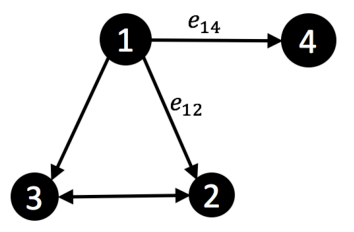
\includegraphics[width=0.3\textwidth]{bilder/social-network-users.png}
	\caption{Verbindungen Nutzer}
	\label{fig:verbindungen-nutzer}
\end{figure}

In Abbildung \vref{fig:verbindungen-nutzer} Nutzer 1 folgt beim Socail Network  gleichzeitig auf die Nutzer 2, 3 und 4 . Es ist jedoch klar, dass Nutzer 1 Benutzer 2 tatsächlich mehr  als Nutzer 4 vertraut, weil Benutzer 1 auch auf 2 und 3 achtet.

\begin{itemize}
\item import application is to suggest  friends to a newcomer, z .B Netflix   is movie and music recommendation systems, where an user is suggested new movies and music basied on his or her rationgs so far.
\item Node( User) classification in social Networks. particular product , and it may be desirable to use the attribute and structural information in the network in order to learn other nodes which may also be interested in the same product. social networks als contain rich information about the content and structure of the network, which may be leveraged of this purpose.( Laut Charu C Seite 10 . an Introduction) z.B.  Zwei Nutzer sind miteinander in einem Socialnetwork verbunden. Es ist wahrscheinlich, dass die Knotenbeschriftungen ebenfalls korreliert sind.
\item Interaktionen  führen  die verschiedenen Akteure in ihrem Verhalten gegenseitig zu beeinflussen. Ein klassisches Beispiel dafür wäre eine virale Marketing Application, bei der wir die Nachrichten zwischen miteinander verbundenen Teilnehmern in einem sozialen Netzwerk nutzen, um die Informationen über die verschiedenen Teile des Netzwerks zu verbreiten
\item Intergrate real-time sensor- based content into dynamic social networks, accelerometers,mobile devices and other GPS-enabled devices, which can be used in a social setting for providing a dynamic and interactive experience
\end{itemize}


\section{Definition vom Social Media}

Laut Turban, Strauss und Lai (2016, S. 8) kann Social Media als Inhalt definiert werden, welcher durch Nutzer, mit Hilfe von Web 2.0 Plattformen, erzeugt wird. Das Erstellen dieser Inhalte dient hierbei laut Turban, Strauss und Lai (2016, S.8) hauptsächlich dazu Meinungen, Erfahrungen und Erkenntnisse auszutauschen.


\section{Welche Konzepte von Social Media können angewendet werden}

\begin{itemize}
\item Verfolgt die Philosophie von miteinander verbundenen Personen (Turban, Strauss und Lai 2016, S. 8)
\item Nutzer generieren, kontrollieren, nutzen und verwalten Inhalte zu geringen
oder keinen kosten (Turban, Strauss und Lai 2016, S. 8)
\item Nutzer stellen den eigentlich bereitgestellten Wert bereit, während Betreiber lediglich eine Plattform anbieten, um dies zu ermöglichen ...
\item Geringe Barrieren für Nutzer, um sich an der Bereitstellung von Inhalten zu
beteiligen ...
\item Hohes Maß an Eigenverwaltung der Nutzer …
\end{itemize}


\section{Enterprise 2.0 (Web 2.0)}


\section{Definition von  e-Commerce}

nach Michael Merz E-Commerce und E-Business, 2. Auflage 2002, dpunkt.verlag Seite 20 lautet  „ die Unterstützung von Handelsaktivitäten über Kommunikationsnetze“, E- Commerce ist der Einsatz von Kommunikationsprotokollen, Sicherheitsinfrastrukturen, digitalem Geld, Electrpmoc Shopping -malls und Datenaustausch…. “


\subsection{Welche Konzepte des eCommerce können angewendet werden}

\begin{itemize}
\item Online Auktionen
\end{itemize}

Aus Hinneburg Kapitel 4 wirtschaftliche Bedeutung von Ebay(Seite 71), „ da nicht die online -Auktionsmärkte selbst, sondern nur ihre Mitglieder Waren zum Verkauf anbieten, entscheidet die jeweilige Mitgliederzahl über die Quantität und Vielfalt des Warenangebotes eines Auktionsmarktes. Andererseits lohnt sich der Verkauf von Waren nur, wenn zahlreiche Käufer den Auktionsmarkt frequentieren.“ er hat noch konkrete beschrieben, wie eine Auktionen lauft.( Seite 72)

In Abbildung \vref{fig:laufende-auktionen} ist die Anzahl der laufenden Auktionen auf den zehn bedeutendsten deutschsprachigen Auktionsmärkten im Internet dargestellt.

\begin{figure}
	\centering
	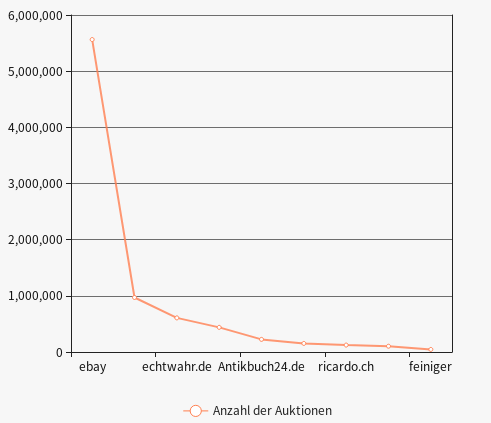
\includegraphics[width=0.7\textwidth]{bilder/laufende-auktionen.png}
	\caption{Laufende Auktionen Quelle: www.auktionssuche.de}
	\label{fig:laufende-auktionen}
\end{figure}

\begin{itemize}
\item gebrauchte Dinge verkaufen
\end{itemize}

Über Ebay Kleinanzeigen verkaufen viele Menschen Dinge, die sie nicht mehr gebrauchen können – mit häufig äußerst kuriosen Anzeigen und witzigen Dialogen.Ein Verkäufer lädt ein Bild vom Objekt mit entsprechenden Informationen wie Maße und Preis hoch. Findet das ein potentieller Käufer interessant, tauschen sich die beiden über weitere Details aus, in den meisten Fällen holt der Käufer das Objekt der Begierde beim Verkäufer ab. Beide Seiten profitieren, denn der Verkäufer hat wieder Platz in der Wohnung und bekommt Geld, der Käufer hat für einen günstigeren Preis sein Wunschobjekt bekommen.

\begin{itemize}
\item Bewertung für die gekaufte Produkte geben
\end{itemize}

bei Amazon kann man nach dem Kaufen eine Bewertung und Kommentare geben, die Bewertung von Stern 1 bis Stern 5, bedeutet das Grad von Unzufrieden bis zufrieden. Die Kommentare sind konkret zu erzählen, die gekaufte Produkte wie gut oder wie schlecht sind.
Bewertung und Kommentare helfen die andere Nutzer auszuwählen.


\section{SocialCommerce}

Socialized Commerce  entwickelt auf Basis von E-Commerce. Laut Turban . (Social Commerce Seite 8 ) :  The figur shows that social Commerce is created from the integration of e- Commerce and e-marketing using  Web 2.0/social Media applications. Es nutzt  mittels sozialer Netzwerke, z.B. Twitter, BLOG,Youtube usw, um Produkte durch soziale Interaktionen und vom Benutzer bereitgestellte Inhalte anzuzeigen, damit  eine  Werbung effektiv erreicht. Es ist ein effektiver Werbekanal für E-Commerce.


\subsection{Welche Konzepte von Social Commerce können angewendet werden}

\begin{itemize}
\item Die Einkaufsnachfrage des Nutzers entstehen unter dem Einfluss von andrem Nutzer. Es besteht eine starke Korrelation zwischen den Bedürfnissen der Nutzer und anderem gekauften Nutzer. „  Word – of- mouth advertising ( Marketing communication) is „ an unpaid form of promotion in which satisfied customers tell other people how much they like a business, product, or Service“, „ Reaserch has revealed that customers are inclined to believe WOM rather than company -generated promotions“ (Laut turban Seite 58), das Interesse und Wunsch werden wegen den von anderen Nutzer geteilt, überprüft und angezeigt Bilder angeregt .
\item Sozial commerce leiten Nutzer an online shops,  der Einkaufsführer ist der Nutzer selbst. Es basiert auf der Erfahrung des Benutzers, Produktinformationen zu teilen, Produkte zu überprüfen, Produkte anzuzeigen und Produkte zu teilen, um mit anderen Nutzern zu interagieren und soziale Beziehungen mit sozialen Attributen herzustellen.
\item Die Plattform erstellt  die Community,  bietet für vielen Online-Shopping-Nutzern einen Ort, um sich miteinande relevante Einkaufsinformationen und Erfahrungen auszutauschen und  mit den gleichen shopping-liebenden Freunden kennenzulernen. Dann die Beziehung werden zwischen die Benutzer verstärken,  Viskosität des Benutzers  und Viskosität zwischen die Webseite und Nutzer zu erhöhen.

\begin{itemize}
\item eine Community-basierte sozialisierte E-Commerce-Plattform wie Facebook, Twitter, etc. Sie implementieren  Präzisions-Marketing
\end{itemize}

\item Gewinnmodell : a, Werbung, 80\% Anteil; b, Kommission; c,  Mehrwertdienste, Sammeln von Beiträgen vom VI, um kostenpflichtige Dienste und spezielle Dienste zu erhalten; d,  Virtueller Warenverbrauch Plug-in-Anwendungsfreigabe von Drittanbietern
\item erweiterte Gewinnmodelle:

\begin{itemize}
\item Social Commerce können Unternehmen helfen, Data Mining und Analyse von Benutzerpräferenzen und potenziellen Bedürfnissen durchzuführen und Online-Werbung für eine bestimmte Zielgruppe zu starten.
\item Sozial Commerce können kostenpflichtige Fragebogenumfragen anbieten und an Umfragen teilnehmen. Die Anzahl der Benutzer, die erhoben werden, um Unternehmen bei der Durchführung von professionellen Ermittlungen und Analysen zu unterstützen
\item Einführung des PPC- und Keyword-Bidding-Service und Einführung des SOLOMO-Modells. Solomo ist ein Akronym für Social Local Mobile ist die soziale, Lokalisierung und mobiles Internet zu verbinden. Kurz gesagt, das SOLOMO-Modell soll lokalisierte Dienste für Benutzer mit gemeinsamen Bedürfnissen über das Internet bereitstellen und effektiv online und offline integrieren.
\end{itemize}

\end{itemize}

Ein wichtiger Faktor im Social Commerce ist das Bild: Website-Betreiber stellen kostenlose, herunterladbare Software bereit, die es den Kunden erleichtert, Fotos hochzuladen und Einkaufserlebnisse auszutauschen. Eine solche Software ermöglicht es den Verbrauchern nicht nur, ihre Lieblingsprodukte aufzulisten, sondern auch die Fotos von Einkaufslisten anzupassen und eine Einnahmequelle  zu schaffen. Zum Beispiel können diese Websites durch den Verkauf von Click-to-Pay-Anzeigen Geld verdienen(nach die Anzahl von Antippen des Nutzer die Kosten rechnen), und sie können auch einige marktrelevante Informationen anbieten.


\section{Welche Konzepte des Online Gamings können angewendet werden}

\begin{itemize}
\item Die Spielteilnehmer kooperieren, um die Aufgabe zu erfüllen. Sie können ein Team bilden, können auch alleine die Aufgabe erfüllen und der Gewinner wird belohnt.
\item Die Spielszene ist wunderschön und Details sind vorhanden.
\item virtuelle Güter verkaufen,  einen gesperrte Kompetenzen geben, sind die Gewinnsquelle von der Spiel Entwicklungsfirma.
\item Es gibt Communities für Gamer, um Nachricht zu veröffentlichen und Erfahrungen auszutauschen. Aus Harald Warmelink, Seite 126
\end{itemize}

\textbf{Literatur :}

Harald warmelink . 2016 Online Gaming and playful Organization 
